\section{MVC+S}


\section{Anwendung in allen View-Komponenten}


\subsection{Dependency-Inversion}


\subsection{Persistence als Service; DAO pattern}

Um den Zugriff auf die Datenbank zu vereinfachen wurde ein Persistenz-Service eingerichtet, sodass der Zugriff transparent geschieht.
Dieser ist nach dem MVC+S implementiert
Siehe Bild \ref{img:mvcps} für eine informelle Graphik der verwendeten Architektur.
Die Persistenz-Service ist modular, sodass Komponenten einfach ausgetauscht werden können.
Dies erreichen wir mithilfe des DAO-Pattern, um den tatsächlichen Zugriff auf den Speicher zu maskieren.
Im Sinne des Dependency-Inversion-Prinzips definiert der \verb|PersistenceService| die DAOs, die dieser benötigt.
Für mehr Information zum Aufbau der Persistenz-Schicht, siehe Kapitel \ref{chap:persistenz}.

Zusätzlich wird ein \verb|DbController| definiert, welcher dafür zuständig ist, die Datenbank zu laden und die DAOs zu instanziieren. Dessen Implementation - und damit die der DAOs - wird über Riverpod injected. Controller erhalten eine Instanz des \verb|PersistenceService| über einen Provider, welcher wiederum einen Provider für den Controller aufruft. Letzterer bestimmt die tatsächliche Implementation.

\begin{figure}[H]
  \centering
  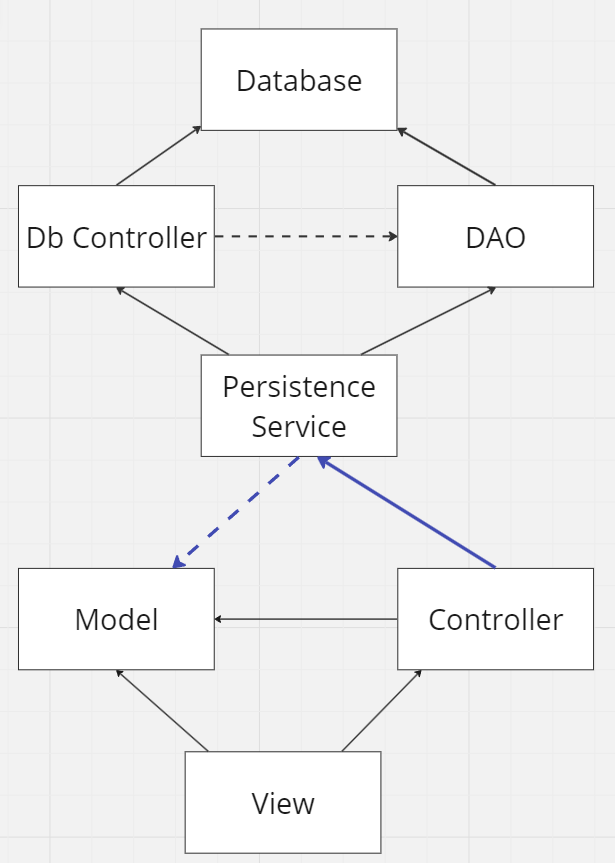
\includegraphics[height=0.5\textwidth]{figures/mvc_p_s.png}
  \caption{MVC+S Architektur}
  \label{img:mvcps}
\end{figure}

\section{Compositum Pattern für FolderItems}


\section{State Management (Riverpod)}


\section{Multi-Language Support}


\section{ErrorHandling}


\subsection{Custom FutureBuilders + null safety}